\documentclass[12pt]{book}

% packages
\usepackage{graphicx}
\usepackage{hyperref}
\usepackage[utf8]{inputenc}
\usepackage{amsmath} % For mathematical equations
\usepackage{import}
\usepackage[greek,english]{babel} % for Greek and English language
\usepackage{alphabeta} % same
\usepackage{multirow,booktabs} % for multirow in tables
\usepackage{amsmath,amsthm,amssymb} % for math formatting
\usepackage[margin=3cm]{geometry} % for page layout
\usepackage[most]{tcolorbox} % for shaded boxes
\usepackage{hyperref} % for hyperlinks
\usepackage{caption} % customizing captions
\usepackage{enumitem} % for list customizations
\usepackage{makecell}	% for a second line in the same table cell
\usepackage{array} % colorbox and arrays inside them
\usepackage{framed}
\usepackage{empheq}
\usepackage{colortbl}	%
\usepackage{fancyhdr}
\usepackage{mathrsfs}
\usepackage{cancel}

% numbering
\usepackage{chngcntr}	% tablenumbering
\counterwithin{table}{subsection}		
\counterwithin{figure}{subsection}	% changes the numbering depth
\numberwithin{equation}{subsection}	% changes the numbering depth

% geometry setup
\geometry{margin=3cm} % uniform margins

% custom colors
\definecolor{bluebox}{RGB}{242,248,253}
\definecolor{redbox}{RGB}{255,242,242}
\definecolor{greenbox}{RGB}{250,255,250}
\definecolor{darkgreenbox}{RGB}{0,85,0}
\definecolor{greybox}{RGB}{247,247,247}
\definecolor{lightgkri}{RGB}{210,210,210}
\definecolor{piolightgkri}{RGB}{249,249,249}
\definecolor{skourogkri}{RGB}{150,150,150}
\definecolor{mavro}{RGB}{0,0,0}

% more on colors
\usepackage{xcolor}
\colorlet{shadecolor}{red!5!white}
\colorlet{framecolor}{red!50!white}																						
\renewenvironment{shaded*}{%
  \def\FrameCommand{\setlength{\FrameRule}{2pt}\fboxsep=\FrameSep \fcolorbox{framecolor}{shadecolor}}%
  \MakeFramed {\advance\hsize-\width \FrameRestore}}%
 {\endMakeFramed}

% box customizations
\newtcolorbox{orismos}[1]{fonttitle=\bfseries,beamer,title=Lower separated,colback=greybox,
title={#1}}

\newtcolorbox[auto counter,number within=subsection]{prdgm}[2][]{%				
enhanced,colback=bluebox,colframe=blue!75!black,fonttitle=\bfseries,breakable,drop fuzzy shadow=black!50!white,				%blue!5!white
title=Παράδειγμα~\thetcbcounter: #2,#1}

\newtcolorbox[auto counter,number within=subsection]{askisi}[2][]{%
enhanced,colback=redbox,colframe=red!95!black,fonttitle=\bfseries,breakable,drop fuzzy shadow=black!50!white,												%red!5!white
title=Άσκηση~\thetcbcounter: #2,#1}

\newtcolorbox[auto counter,number within=section]{ergasia}[2][]{%
enhanced,colback=white,colframe=black!95!white,fonttitle=\bfseries,breakable,drop fuzzy shadow=black!50!white,
title=Εργασία~\thetcbcounter: #2,#1}


% custom captions
\captionsetup[table]{name=Πίνακας}
\captionsetup[figure]{name=Εικόνα}

% miscellaneous
\usepackage{xfrac} % for tipped over fractions
\setlength{\parindent}{0pt} % for no indentation for paragraphs


% some unit shortcuts
\newcommand{\monm}{\text{ }$m$\text{ }}
\newcommand{\mons}{\text{ }$s$\text{ }}
\newcommand{\monkg}{\text{ }$Kg$\text{ }}
\newcommand{\monms}{\text{ }$\sfrac{m}{s}$\text{ }}
\newcommand{\monmss}{\text{ }$\sfrac{m}{s^2}$\text{ }}
\newcommand{\monN}{\text{ }$N$\texxt{ }}
\newcommand{\monJ}{\text{ }$J$\text{ }}
\newcommand{\monW}{\text{ }$W$\text{ }}





% Custom Greek translations for specific captions
\addto\captionsenglish{
    \renewcommand{\chaptername}{Κεφάλαιο}
    \renewcommand{\contentsname}{Περιεχόμενα}
}




% Document Metadata
\title{Φυσική Α' Λυκείου}
\author{Δρ Στυλιανός Καρύδας}

\begin{document}


\maketitle % Title page
\tableofcontents % Table of contents



% Include chapters
\chapter{Εισαγωγικές Έννοιες}
\clearpage
%
%
%
%						MONOMETRA KAI DIANISMATIKA MEGETHI
%
%
%
\section{Μονόμετρα και Διανυσματικά Μεγέθη}

Στη Φυσική του Λυκείου, υπάρχουν δύο είδη φυσικών μεγεθών που θα μας απασχολήσουν, τα μονόμετρα και τα διανυσματικά μεγέθη.

\begin{orismos}{Μονόμετρα Μεγέθη:}
Είναι τα μεγέθη που ορίζονται μόνο από την τιμή τους (δηλαδή το μέτρο τους).\\
\textit{Μερικά μονόμετρα μεγέθη είναι η μάζα, ο χρόνος, το ηλεκτρικό φορτίο κ.α.}
\end{orismos}
\vspace{4mm}
\begin{orismos}{Διανυσματικά Μεγέθη:}
Είναι τα μεγέθη που για να οριστούν χρειάζεται τόσο η τιμή τους (δηλαδή το μέτρο τους), όσο και η κατεύθυνσή τους.
\tcblower
Κατεύθυνση ονομάζουμε μαζί τη διεύθυνση και τη φορά ενός διανύσματος. Διεύθυνση είναι η ευθεία πάνω στην οποία βρίσκεται το διάνυσμα, ενώ φορά είναι το άκρο της, προς το οποίο είναι στραμμένο.\\
\textit{Μερικά διανυσματικά μεγέθη είναι: όλες οι δυνάμεις, η ταχύτητα, κ.α.}
\end{orismos}

\vspace{2mm}
Για να αναπαραστήσουμε ένα διανυσματικό μέγεθος, χρησιμοποιούμε ένα διάνυσμα (βέλος), δηλαδή ένα \textit{προσανατολισμένο ευθύγραμμο τμήμα}. Καθώς τα διανυσματικά μεγέθη χρειάζονται τόσο μέτρο, όσο και κατεύθυνση για να οριστούν, είναι επόμενο, όταν τα συγκρίνουμε, να πρέπει να λάβουμε υπ'όψη και τα δύο. Σε ένα διάνυσμα, λοιπόν, η κατεύθυνση του βέλους ταυτίζεται με την κατεύθυνση του διανυσματικού μεγέθους που απεικονίζει, ενώ το \textit{μήκος} του διανύσματος αναπαριστά το \textit{μέτρο} του μεγέθους.
\vspace{2mm}

\begin{orismos}{Ομόρροπα-Αντίρροπα Διανύσματα}
Δύο διανύσματα ονομάζονται ομόρροπα όταν έχουν ίδια κατεύθυνση (δηλαδή ίδια διεύθυνση και φορά), ενώ ονομάζονται αντίρροπα όταν έχουν αντίθετη κατεύθυνση (δηλαδή ίδια διεύθυνση αλλά ανάποδη φορά).
\begin{center}
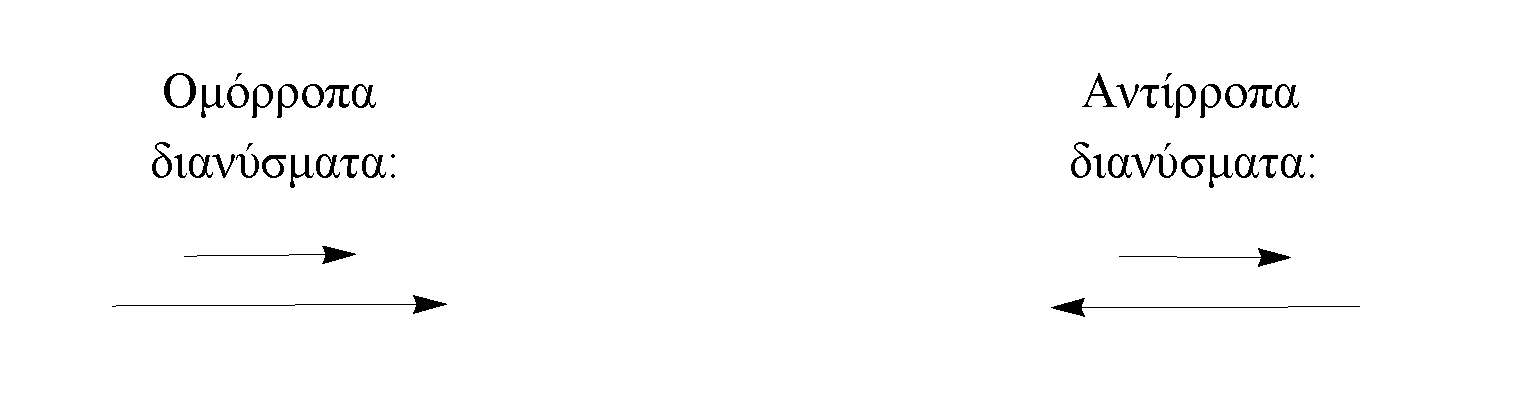
\includegraphics[width=0.95\linewidth]{images/dianismata2.pdf}
\end{center}
\end{orismos}
\vspace{2mm}
Έχοντας αυτό κατά νου, μπορούμε να καθορίσουμε τη σχέση δύο διανυσμάτων μεταξύ τους, τόσο με βάση το μέτρο τους, όσο και με βάση την κατεύθυνσή τους.
\vspace{2mm}
\begin{orismos}{Ίσα-Αντίθετα Διανύσματα}
Δύο διανύσματα ονομάζονται \textbf{ίσα}, όταν είναι ομόρροπα \textit{και} έχουν ίσα μέτρα.\\
Δύο διανύσματα ονομάζονται \textbf{αντίθετα}, όταν είναι αντίρροπα \textit{και} έχουν ίσα μέτρα.
\tcblower
Δύο διανύσματα \textbf{δεν} είναι ίσα, σε κάθε άλλη περίπτωση. Δηλαδή αν τα μέτρα τους είναι διαφορετικά ή αν έχουν διαφορετική κατεύθυνση, ακόμα και αν έχουν ίσα μέτρα, τότε \textbf{δεν} είναι ίσα!
\end{orismos}
\vspace{2mm}
\begin{prdgm}{Σύγκριση Διανυσμάτων}
Όλα τα παρακάτω διανύσματα έχουν το ίδιο μήκος. Να σημειώσετε αν είναι ίσα, αντίθετα ή τίποτα από τα δύο.
\tcblower
\begin{center}
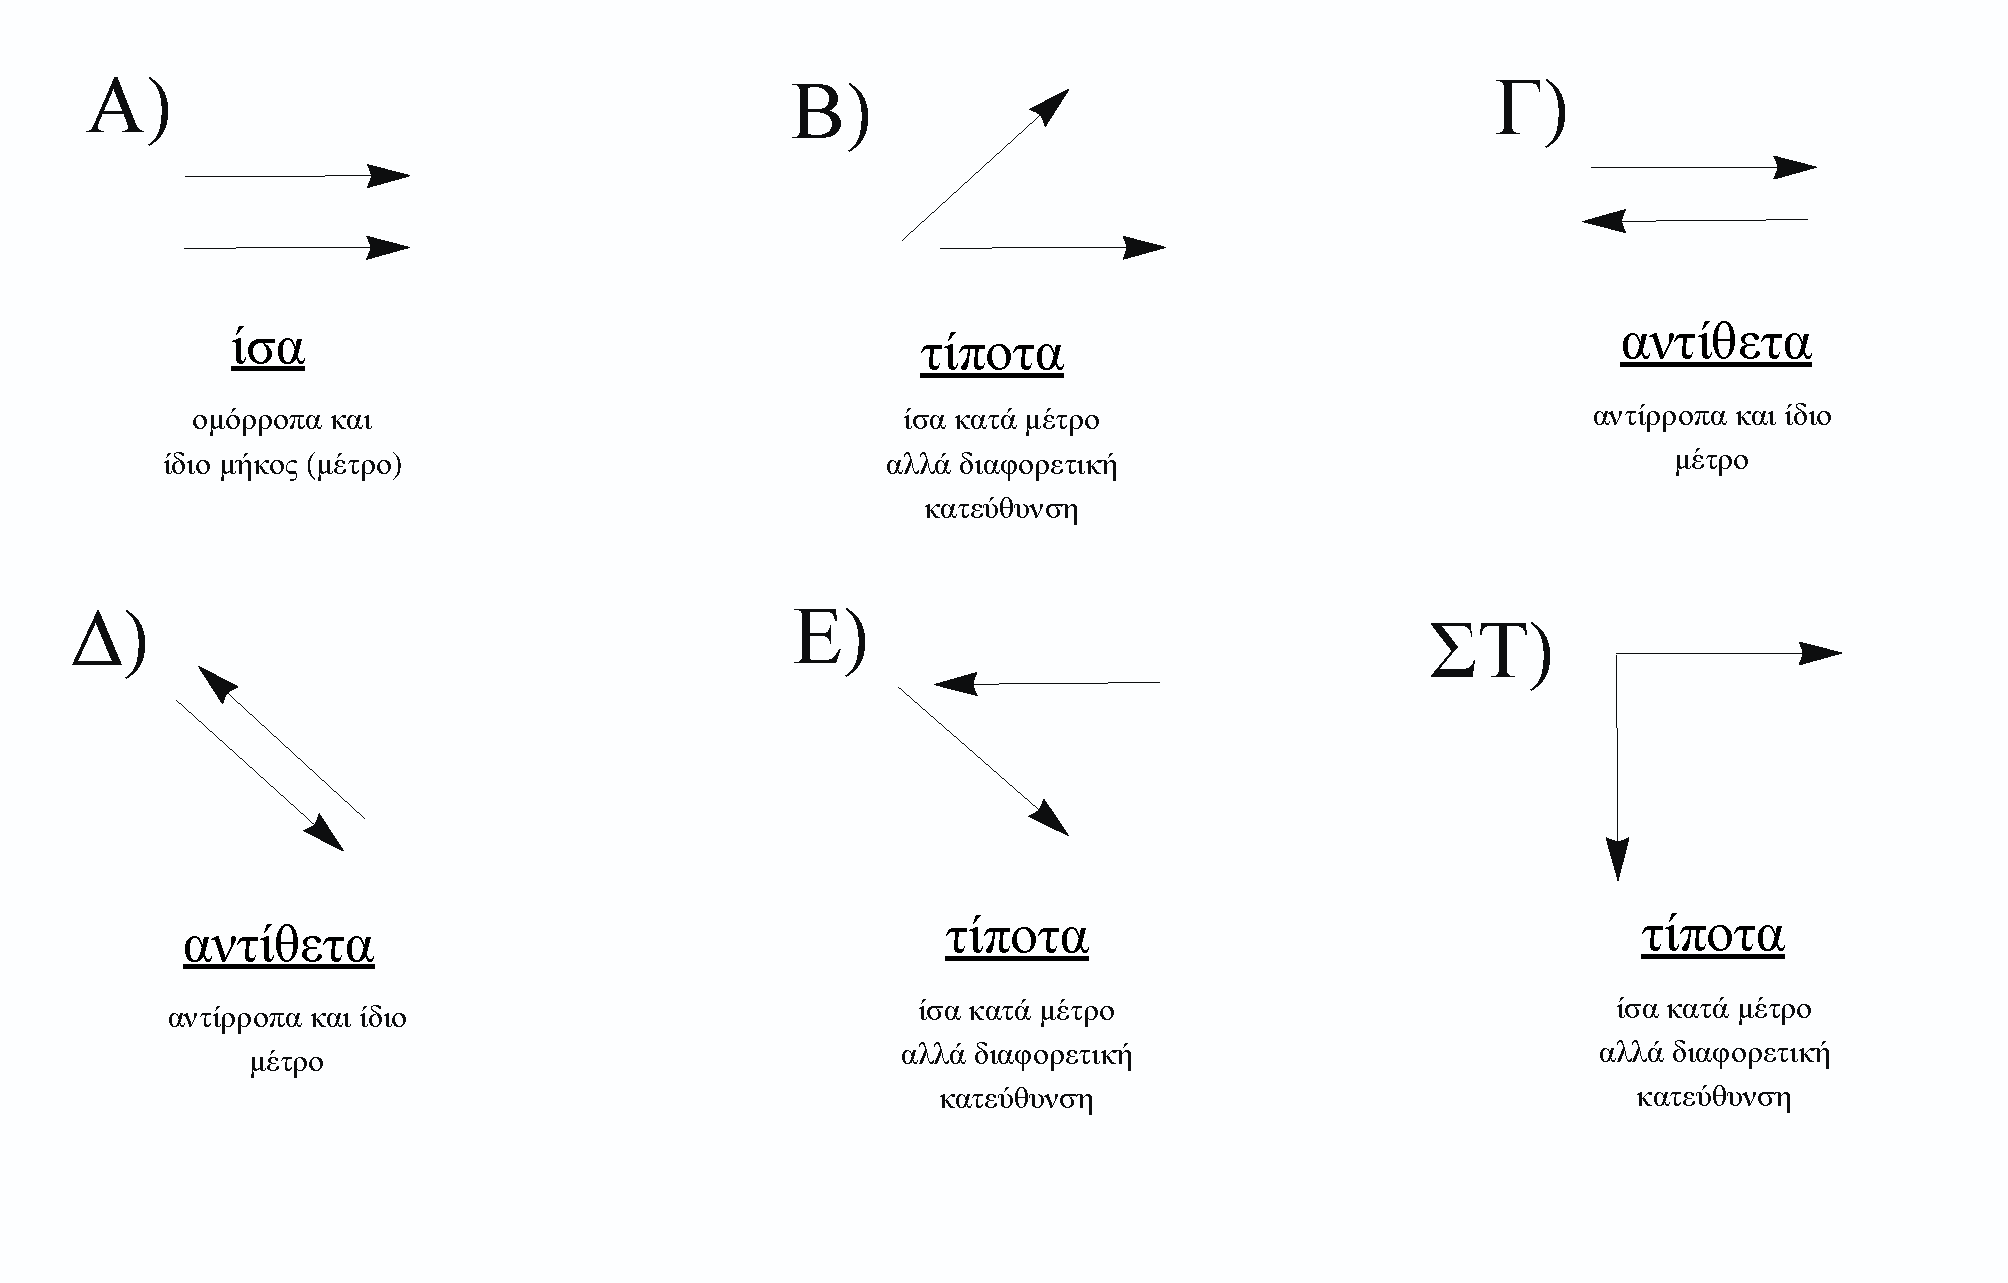
\includegraphics[width=0.95\linewidth]{images/dianismata1.pdf}
\end{center}
\end{prdgm}
%
%
%
%																	Monades Metrisis
%
%
%
\clearpage
\section{Μονάδες Μέτρησης -\\ Διεθνές Σύστημα Μονάδων (SI)}

Για να εκφράσουμε οποιοδήποτε φυσικό μέγεθος, είτε μονόμετρο είτε διανυσματικό, χρειαζόμαστε μια μονάδα σε σύγκριση με την οποία το μετράμε. Για παράδειγμα, όταν λέμε ότι μια μάζα είναι ίση με $2 \text{ }Kg$, εννοούμε ότι είναι διπλάσια από τη μονάδα μάζας που έχουμε ονομάσει $1 \text{ }Kg$.

Ανάλογα με το αντικείμενο όμως που μελετάμε, δεν είναι πάντα χρήσιμο το να εκφράζουμε τη μάζα σε $Kg$. Επομένως, για οποιοδήποτε φυσικό μέγεθος μπορούμε να ορίσουμε πολλές μονάδες με βάση τις οποίες το εκφράζουμε. Στην περίπτωση της μάζας, άλλες μονάδες είναι για παράδειγμα το γραμμάριο $(gr)$, ο τόνος $(tn)$ κλπ.

Όμως η ύπαρξη πολλών μονάδων, μπορεί με τη σειρά της να δημιουργήσει σύγχυση όταν εκφράζεται κάποιο φυσικό μέγεθος. Για το λόγο αυτό, έχει δημιουργηθεί το \textit{Διεθνές Σύστημα Μονάδων, (SI)}, στο οποίο όλα τα φυσικά μεγέθη είναι υποχρεωτικό να εκφράζονται με βάση συγκεκριμένες μονάδες.

Παρακάτω παρουσιάζουμε έναν πίνακα με όλα τα μεγέθη που θα χρησιμποιήσουμε φέτος, το γράμμα που χρησιμοποιούμε συνήθως για να τα συμβολίσουμε, το είδος του μεγέθους (με \textbf{Μ} θα συμβολίζουμε τα μονόμετρα μεγέθη και με \textbf{Δ} τα διανυσματικά) και τις αντίστοιχες μονάδες τους στο SI.
\begin{table}[h!]
\begin{center}
\tcbox[left=0mm,right=0mm,top=0mm,bottom=0mm,boxsep=0mm,
toptitle=0.5mm,bottomtitle=0.5mm,center title,title=Πίνακας Φυσικών Μεγεθών,colframe=black,colback=white,enhanced,breakable,drop fuzzy shadow=black!50!white]{%
%\arrayrulecolor{white!50!black}\renewcommand{\arraystretch}{1.2}%
\begin{tabular}{ | l | c | c | c |}
  \hline
 \rowcolor{lightgkri} \textbf{Μέγεθος} & \textbf{Σύμβολο} & \textbf{Είδος} & \textbf{Μονάδα στο SI} \\ 
  \hline	
 \textbf{Χρόνος} & $t$ & \textbf{M} & \multirow{2}{8em}{\makecell{sec}} \\
 \textbf{Χρον. Διάστημα} & $Δt$ & \textbf{M} & \\ 
	\hline
	\textbf{Θέση} & $x$ & \textbf{Δ} & \multirow{3}{*}{m} \\ 
	\textbf{Μετατόπιση} & $Δx$ & \textbf{Δ} &  \\ 
	\textbf{Διάστημα} & $S$ & \textbf{M} & \\
\hline
	\textbf{Ταχύτητα} & $v$ & \textbf{Δ} & \multirow{2}{8em}{\makecell{$\sfrac{\text{\normalsize{m}}}{\text{\normalsize{s}}}$}}\\ 
	\textbf{Μέση Ταχύτητα} & $v_\mu$ & \textbf{M} &\\
  \hline
		\textbf{Επιτάχυνση} & $a$ & \textbf{Δ} & \makecell{$\sfrac{\text{\normalsize{m}}}{\text{\normalsize{s}}^2}$} \\
	\hline
		\textbf{Μάζα} & $m$ & \textbf{M} & Kg \\
	\hline
		\textbf{Δύναμη} & $F$ & \textbf{Δ} & N \\
	\hline
		\textbf{Έργο} & $W$ & \textbf{M} & \multirow{2}{*}{J}\\
		\textbf{Ενέργεια} & $E$ & \textbf{M} & \\
	\hline
		\textbf{Ισχύς} & $P$ & \textbf{M} & W \\
	\hline
\end{tabular}}
\end{center}
\caption{}
\label{PinMonadon1}
\end{table}


\section{Υποδιαιρέσεις και Πολλαπλάσια των βασικών μονάδων}

Κατά τη μέτρηση των διαφόρων μεγεθών, μπορούμε να χρησιμοποιήσουμε υποδιαιρέσεις και πολλαπλάσια των βασικών μονάδων του SI που παρουσιάστηκαν στον Πίνακα \ref{PinMonadon1}. Οι υποδιαιρέσεις και τα πολλαπλάσια των βασικών μονάδων βασίζονται, ως επί το πλείστον, στις δυνάμεις του 10, όπως φαίνεται στον Πίνακα \ref{PinIpodiaireseon}

\begin{table}[h!]
\begin{center}
\tcbox[left=0mm,right=0mm,top=0mm,bottom=0mm,boxsep=0mm,
toptitle=0.5mm,bottomtitle=0.5mm,center title,title=Υποδιαιρέσεις-Πολλαπλάσια,colframe=black,colback=white,enhanced,breakable,drop fuzzy shadow=black!50!white]{%
\begin{tabular}{ | c | c | c | c | }
  \hline
 \rowcolor{lightgkri} Σύμβολο & Δύναμη του 10 & Σύμβολο & Δύναμη του 10 \\ 
  
	G (Giga) & $10^9$ & d (deci) & $10^{-1}$ \\
	\hline
  M (Mega) & $10^6$ & c (centi) & $10^{-2}$\\ 
  \hline
  K (Kilo) & $10^3$ & m (mili) & $10^{-3}$\\ 
  \hline
  
\end{tabular}}
\end{center}
\caption{}
\label{PinIpodiaireseon}
\end{table}

\noindent \begin{minipage}{0.6\textwidth}
\vspace{1cm}
\tcbox[colback=mavro,colframe=mavro,
left=0mm,right=0mm,top=0mm,bottom=0mm,boxsep=1mm,boxrule=0.5pt,enhanced,breakable,drop fuzzy shadow=black!50!white,center title,
title=\Large{ΜΗΚΟΣ}]{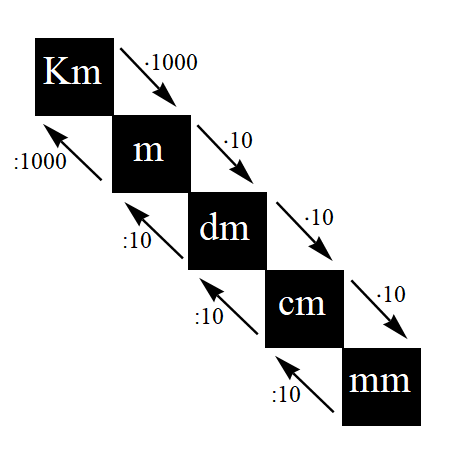
\includegraphics[width=\textwidth]{images/metatropesmikos2.png}}%
\captionof{figure}{}
\label{metatropesmikos}
\end{minipage}
\hspace{0.05\textwidth}
\begin{minipage}{0.35\textwidth}
Με βάση αυτόν τον Πίνακα μπορούμε να βρούμε πολλαπλάσια και υποδιαιρέσεις για όλες τις μονάδες, ανεξάρτητα από το αν ανήκουν στο SI. Για παράδειγμα, στην περίπτωση του μήκους, του οποίου η μονάδα στο SI είναι το $1 m$, εργαζόμαστε όπως στην περίπτωση της Eικόνας \ref{metatropesmikos}. Όμως, για κάποια μεγέθη, υπάρχουν και υποδιαιρέσεις που δεν ακολουθούν απαραίτητα τον Πίνακα \ref{PinIpodiaireseon}.  Δύο τέτοια παραδείγματα που θα μας απασχολήσουν είναι η μάζα και ο χρόνος, που μετατρέπονται με βάση τις Εικόνες \ref{metatropesmaza} και \ref{metatropeshronos} αντίστοιχα.
\end{minipage}

\noindent \begin{minipage}{0.45\textwidth}
\vspace{1cm}
\tcbox[colback=mavro,colframe=mavro,
left=0mm,right=0mm,top=0mm,bottom=0mm,boxsep=1mm,boxrule=0.5pt,center title,enhanced,breakable,drop fuzzy shadow=black!50!white,
title=\Large{ΜΑΖΑ}]{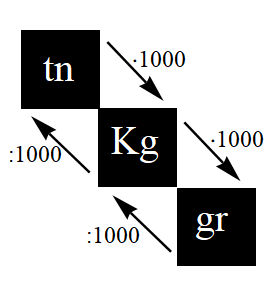
\includegraphics[width=\textwidth]{images/metatropesmaza2.png}}%
\captionof{figure}{}
\label{metatropesmaza}
\end{minipage}
\hspace{0.1\textwidth}
\begin{minipage}{0.45\textwidth}
\vspace{1cm}
\tcbox[colback=mavro,colframe=mavro,
left=0mm,right=0mm,top=0mm,bottom=0mm,boxsep=1mm,boxrule=0.5pt,center title,enhanced,breakable,drop fuzzy shadow=black!50!white,
title=\Large{ΧΡΟΝΟΣ}]{%
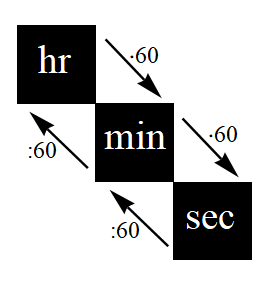
\includegraphics[width=\textwidth]{images/metatropeshronos2.png}}
\captionof{figure}{}
\label{metatropeshronos}
\end{minipage}

\begin{prdgm}[halign=flush left,label=prdgm:metatropesmonadon]{Μετατροπές Βασικών Μονάδων}
\textbf{Να μετατρέψετε τις παρακάτω μονάδες όπως ζητείται σε κάθε περίπτωση.}
\tcblower


$\vspace{4mm}\mathbf{
0,7 \text{ }Km \xrightharpoonup{m}} \text{ }0,7 \cdot 1000 \monm = 700 \monm\\
$
\vspace{4mm}
$\mathbf{
240 \text{ }cm \xrightharpoonup{Km}} \text{ }240 : 100.000 \text{ Km } = 0,0024 \text{ Km }\\
$
\vspace{4mm}
$\mathbf{
0,5 \text{ }Kg \xrightharpoonup{gr}} \text{ }0,5 \cdot 1.000 \text{ gr }= 500 \text{ gr }\\
$
\vspace{4mm}
$\mathbf{
0,12\text{ } m \xrightharpoonup{mm}} \text{ }0,12 \cdot 1.000 \text{ mm } = 120 \text{ mm }\\
$
\vspace{4mm}
$\mathbf{
525 \text{ }gr \xrightharpoonup{Kg}} \text{ }525: 1.000 \monkg= 0.525 \monkg\\
$
\vspace{4mm}
$\mathbf{
220 \text{ }dm \xrightharpoonup{Km}}\text{ } 220:10.000 \text{ Km } = 0,022 \text{ Km }\\
$
\vspace{4mm}
$\mathbf{
3 \text{ }min \xrightharpoonup{sec}} \text{ } 3 \cdot 60 \mons = 180 \mons\\
$
\vspace{4mm}
$\mathbf{
0,1\text{ } hr \xrightharpoonup{min}} \text{ } 0,1 \cdot \text{ min }= 6 \text{ min }\\
$


\end{prdgm}

\subsection{Μετατροπές Σύνθετων Μονάδων - Ταχύτητα}
Είναι επιπλέον δυνατό, να μετατρέψουμε σύνθετες μονάδες, όπως για παράδειγμα η ταχύτητα. Για να το κάνουμε αυτό μετατρέπουμε ξεχωριστά κάθε μια από τις βασικές μονάδες που συναποτελούν τη σύνθετη μονάδα, όπως στο Παράδειγμα \ref{prdgm:metatropestahititas} που ακολουθεί.
\vspace{4mm}
\begin{prdgm}[halign=flush left,label=prdgm:metatropestahititas]{Μετατροπές Ταχύτητας}
\textbf{Να μετατρέψετε τις παρακάτω ταχύτητες.}
\tcblower

$\vspace{2mm}
\mathbf{
72 }\text{ }\sfrac{\mathbf{Km}}{\mathbf{h}}
\xrightharpoonup{\sfrac{\mathbf{m}}{\mathbf{s}}} \text{ }72 \cdot \frac{1.000 \text{ }m}{3.600\text{ }s}=\frac{72.000 \text{ }m}{3.600\text{ }s}=20 \text{ }{\sfrac{m}{s}}$\\
\vspace{2mm}
$
\mathbf{
9 }\text{ }\sfrac{\mathbf{Km}}{\mathbf{h}}
\xrightharpoonup{\sfrac{\mathbf{m}}{\mathbf{s}}} \text{ }9 \cdot \frac{1.000 \text{ }m}{3.600\text{ }s}=\frac{9.000 \text{ }m}{3.600\text{ }s}=2,5 \text{ }{\sfrac{m}{s}}$\\
\vspace{2mm}
$\mathbf{
40 }\text{ }\sfrac{\mathbf{m}}{\mathbf{s}}
\xrightharpoonup{\sfrac{\mathbf{Km}}{\mathbf{h}}} \text{ }40 \cdot \frac{\frac{1}{1.000} \text{ }Km}{\frac{1}{3.600}\text{ }h}=40\cdot\frac{3.600 \text{ }Km}{1.000\text{ } h}=144 \text{ }{\sfrac{Km}{h}}$\\
\vspace{2mm}
$\mathbf{
2 }\text{ }\sfrac{\mathbf{m}}{\mathbf{s}}
\xrightharpoonup{\sfrac{\mathbf{Km}}{\mathbf{h}}} \text{ }2 \cdot \frac{\frac{1}{1.000} \text{ }Km}{\frac{1}{3.600}\text{ }h}=2\cdot\frac{3.600 \text{ }Km}{1.000\text{ } h}=7,2 \text{ }{\sfrac{Km}{h}}$\\
\vspace{2mm}
$\mathbf{
120 }\text{ }\sfrac{\mathbf{Km}}{\mathbf{h}}
\xrightharpoonup{\sfrac{\mathbf{m}}{\mathbf{min}}} \text{ }120 \cdot \frac{1.000 \text{ }m}{60 min}=\frac{120.000 \text{ }m}{60 \text{ }min}=2.000 \text{ } \sfrac{m}{min}$\\

\end{prdgm}

\noindent \begin{minipage}{0.45\textwidth}
\vspace{1cm}
\tcbox[colback=mavro,colframe=mavro,
left=0mm,right=0mm,top=0mm,bottom=0mm,boxsep=1mm,boxrule=0.5pt,enhanced,breakable,drop fuzzy shadow=black!50!white,center title,
title=\Large{ΤΑΧΥΤΗΤΑ}]{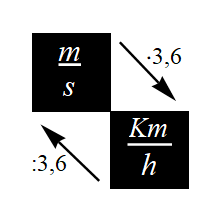
\includegraphics[width=\textwidth]{images/metatropestahitita.png}}%
\captionof{figure}{}
\label{metatropestahitita}
\end{minipage}
\hspace{0.05\textwidth}
\begin{minipage}{0.45\textwidth}
Η μετατροπή ταχύτητας $\sfrac{\large{m}}{\large{s}}\rightleftharpoons \sfrac{\large{Km}}{\large{h}}$, αν και δεν είναι η μόνη πιθανή, θα είναι αυτή που θα συναντήσουμε πιο συχνά. Γι' αυτό, μπορούμε να απομνημονεύσουμε τον κανόνα που παρουσιάζεται στην Εικόνα \ref{metatropestahitita}, αποφεύγοντας τη διαδικασία που παρουσιάζεται στο Παράδειγμα \ref{prdgm:metatropestahititas}.
\end{minipage}

\begin{shaded*}
\underline{ΠΡΟΣΟΧΗ}: Πριν χρησιμοποιήσουμε οποιονδήποτε τύπο, πρέπει να βεβαιωνόμαστε ότι όλα τα μεγέθη βρίσκονται στις μονάδες που επιθυμούμε, οι οποίες συνήθως είναι αυτές του SI. Αν δεν ισχύει αυτό, τότε το αποτέλεσμα του τύπου \textbf{θα είναι λάθος!}\\
\textit{\underline{π.χ.:} Aν μια άσκηση δίνει ταχύτητα $v=36 \text{ }\sfrac{km}{h}$ και χρονικό διάστημα $\Delta t=3 \text{ }sec$, αυτά τα μεγέθη \textbf{δεν} είναι σωστό να χρησιμοποιηθούν απευθείας στον τύπο $\Delta x=v\cdot \Delta t$.}
\end{shaded*}


\vspace{4mm}
\begin{askisi}[halign=flush left,label=ask:metatropesmonadon]{Μετατροπές Μονάδων}
\textbf{Να μετατρέψετε τις παρακάτω μονάδες όπως ζητείται σε κάθε περίπτωση.}
\tcblower
\vspace{1mm}

$\mathbf{
12 \text{ }Km \xrightharpoonup{m}}\\
$

$\mathbf{
15 }\text{ }\sfrac{\mathbf{m}}{\mathbf{s}}
\xrightharpoonup{\sfrac{\mathbf{Km}}{\mathbf{h}}}$\\

$\mathbf{
24 \text{ }dm \xrightharpoonup{cm}}\\
$

$\mathbf{
350\text{ }mm \xrightharpoonup{Km}}\\
$

$\mathbf{
16.200 \text{ } gr \xrightharpoonup{Kg}}\\
$

$
\mathbf{
18 }\text{ }\sfrac{\mathbf{Km}}{\mathbf{h}}
\xrightharpoonup{\sfrac{\mathbf{m}}{\mathbf{s}}}$\\

$\mathbf{
30 \text{ }sec \xrightharpoonup{min}}\\
$

$\mathbf{
6 \text{ }min \xrightharpoonup{sec}}\\
$

$
\mathbf{
36 }\text{ }\sfrac{\mathbf{Km}}{\mathbf{h}}
\xrightharpoonup{\sfrac{\mathbf{m}}{\mathbf{s}}}$\\

$\mathbf{
30 }\text{ }\sfrac{\mathbf{m}}{\mathbf{s}}
\xrightharpoonup{\sfrac{\mathbf{Km}}{\mathbf{h}}}$\\

$\mathbf{
20\text{ } Kg \xrightharpoonup{gr}}\\
$

$\mathbf{
1800 \text{ } min \xrightharpoonup{hr}}\\
$


$\mathbf{
7200 \text{ }sec \xrightharpoonup{hr}}\\
$

\end{askisi}


\clearpage

\section{Εργασίες για το Σπίτι:}
\begin{ergasia}{Ορισμοί (Θεωρία)}
Να συμπληρώσετε και να \underline{μάθετε} τους παρακάτω ορισμούς:
\tcblower
\textbf{Μονόμετρα Μεγέθη} είναι\\

\vspace{1.6cm}

\textbf{Διανυσματικά Μεγέθη} είναι\\

\vspace{1.6cm}

\textbf{Ομόρροπα} ονομάζονται δύο διανύσματα όταν\\

\vspace{1.6cm}

\textbf{Αντίρροπα} ονομάζονται δύο διανύσματα όταν\\

\vspace{1.6cm}

\textbf{Ίσα} ονομάζονται δύο διανύσματα όταν\\

\vspace{1.6cm}

\textbf{Αντίθετα} ονομάζονται δύο διανύσματα όταν\\

\vspace{1.6cm}
\end{ergasia}

\clearpage

\begin{ergasia}{Μεγέθη και σύμβολα-μονάδες (Θεωρία)}
\textbf{Να συμπληρώσετε τον παρακάτω πίνακα:}

\begin{center}
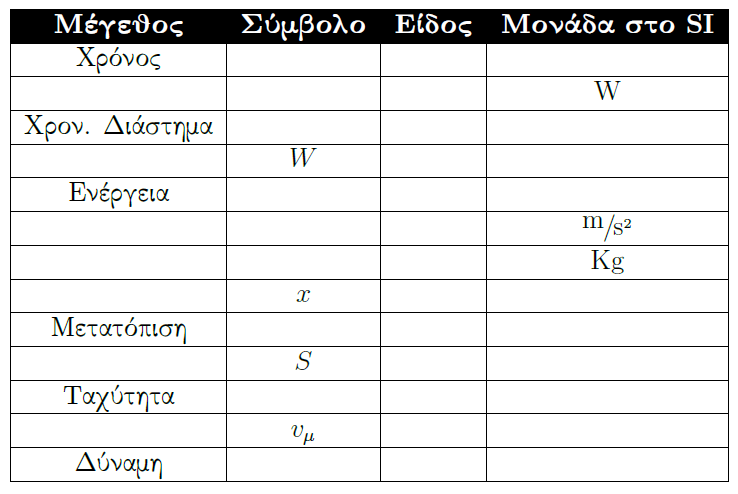
\includegraphics[width=0.7\textwidth]{images/pinakasaskisis.png}
\end{center}

\end{ergasia}


\vspace{4mm}
\begin{ergasia}{Μετατροπές Μονάδων}
\textbf{Να γίνουν οι παρακάτω μετατροπές.}
\tcblower

$\mathbf{
6 \text{ }dm \xrightharpoonup{mm}}\\
$

$\mathbf{
520 \text{ } gr \xrightharpoonup{Kg}}\\
$

$
\mathbf{
18 }\text{ }\sfrac{\mathbf{Km}}{\mathbf{h}}
\xrightharpoonup{\sfrac{\mathbf{m}}{\mathbf{s}}}$\\

$\mathbf{
0,2 \text{ }hrs \xrightharpoonup{sec}}\\
$

$
\mathbf{
360 }\text{ }\sfrac{\mathbf{Km}}{\mathbf{h}}
\xrightharpoonup{\sfrac{\mathbf{m}}{\mathbf{s}}}$\\

$\mathbf{
80 }\text{ }\sfrac{\mathbf{m}}{\mathbf{s}}
\xrightharpoonup{\sfrac{\mathbf{Km}}{\mathbf{h}}}$\\

$\mathbf{
500 \text{ } min \xrightharpoonup{hr}}\\
$

$\mathbf{
0,09 \text{ }Kg \xrightharpoonup{gr}}\\
$

$\mathbf{
5.400 \text{ }sec \xrightharpoonup{hr}}\\
$

\end{ergasia}

%\end{document}

 % Automatically adds .tex
%\include{chapters/book2} % Automatically adds .tex

\end{document}
